\documentclass{beamer}
\usepackage{amssymb}
\setbeamertemplate{navigation symbols}{}
\setbeamertemplate{footline}[page number]
\usepackage{amsmath}
\usepackage{amsrefs}
\usepackage{graphicx}
\usepackage{bookman}
\usepackage{url}
\usepackage{amsthm}
\usepackage{verbatim}
\usepackage{xcolor}
\bibliographystyle{amsmath}
\usetheme{Madrid}
\usecolortheme{dolphin}
\useoutertheme[footline=authortitle]{miniframes}


\title[\#FriendFinder]{\#FriendFinder: On-Campus Social Networking}
\author[Allen]{Tyler Allen\\ \footnotesize Western Carolina University}

\begin{document}

%\setbeamercolor{title}
\section{Introduction}
\begin{frame}
\begin{center}
\maketitle
\end{center}
\end{frame}

\begin{frame}{Outline}
Today we will:
\begin{itemize}
\item Discuss the purpose of this application.
\item View the technologies used in the creation of this application.
\item View the design and current implementation progress of this application.
\end{itemize}
\end{frame}

\begin{frame}{Purpose and Goals}
\begin{itemize}
\item Develop a social-networking application for college students.
\item Target the application at specific campuses.
\item Provides features targeted at users with low geographical distance between them.
\end{itemize}
\end{frame}

\begin{frame}{Features for Users}
\begin{itemize}
\item User Accounts and Profiles
\item Friends
\item Events
\item Groups
\item Calendars
\item Mapping Locations
\end{itemize}
\end{frame}

\begin{frame}{Technologies}
\begin{itemize}
\item Implementation Language: Java
\item Application Platform: Android
\item Network Encryption via Secure Socket Layer (SSL)
\item Network Communication using Javascript Object Notation (JSON)
\item Database Communication using Java Database Connectivity (JDBC)
\item Backend Database using PostgreSQL
\item Client Side Database using SQLite3
\end{itemize}
\end{frame}

\section{Platforms and Technologies}
\begin{frame}{Java}
\begin{itemize}
\item Standard Language for Android
\item Solid Server Language
\item Built-in Database Connectivity
\item Using the same language for the whole project simplifies development.
\end{itemize}
C/C++ were considered, but would increase development time drastically.
\end{frame}

\begin{frame}{Android}
\begin{itemize}
\item Android is one of the most popular mobile platforms in the world.
\item Prior experience in both Java and Android
\item Majority of available testing devices were Android.
\end{itemize}
\end{frame}

\begin{frame}{Secure Socket Layer}
\begin{itemize}
\item Encryption is necessary for any system with private user data.
\item SSL provides encryption for all data sent between client and server.
\item SSL is recommended by Android.
\item SSL support is built into the Android Framework.
\item Hypertext Transfer Protocol Secure (HTTPS) could be placed on top of SSL in the future if 
necessary (e.g. for a web application).
\end{itemize}
\end{frame}

\begin{frame}{JSON}
\begin{itemize}
\item Key-value store.
\item Built for server-client communication within web applications.
\item Built-in Android support.
\item Multiple supported Java libraries.
\end{itemize}
\end{frame}

\begin{frame}{JDBC and PostgreSQL}
\begin{itemize}
\item JDBC is the default library for accessing databases in Java.
\item PostgreSQL is open-source and has JDBC support.
\item Prior experience using PSQL for designing a web application.
\end{itemize}
\end{frame}

\begin{frame}{Client-side Databases}
\begin{itemize}
\item The Android Framework uses \emph{ContentProvider}s to store large volumes of data.
\item SQLite3 is the Android supported database language compatible with \emph{ContentProvider}s.
\item SQLite is lighter weight than PostgreSQL, and provides less features, but is suitable for the
reduced amount of data stored on each individual client.
\end{itemize}
\end{frame}

\section{Design}
%\begin{frame}{Android Storyboard}
%\begin{center}
%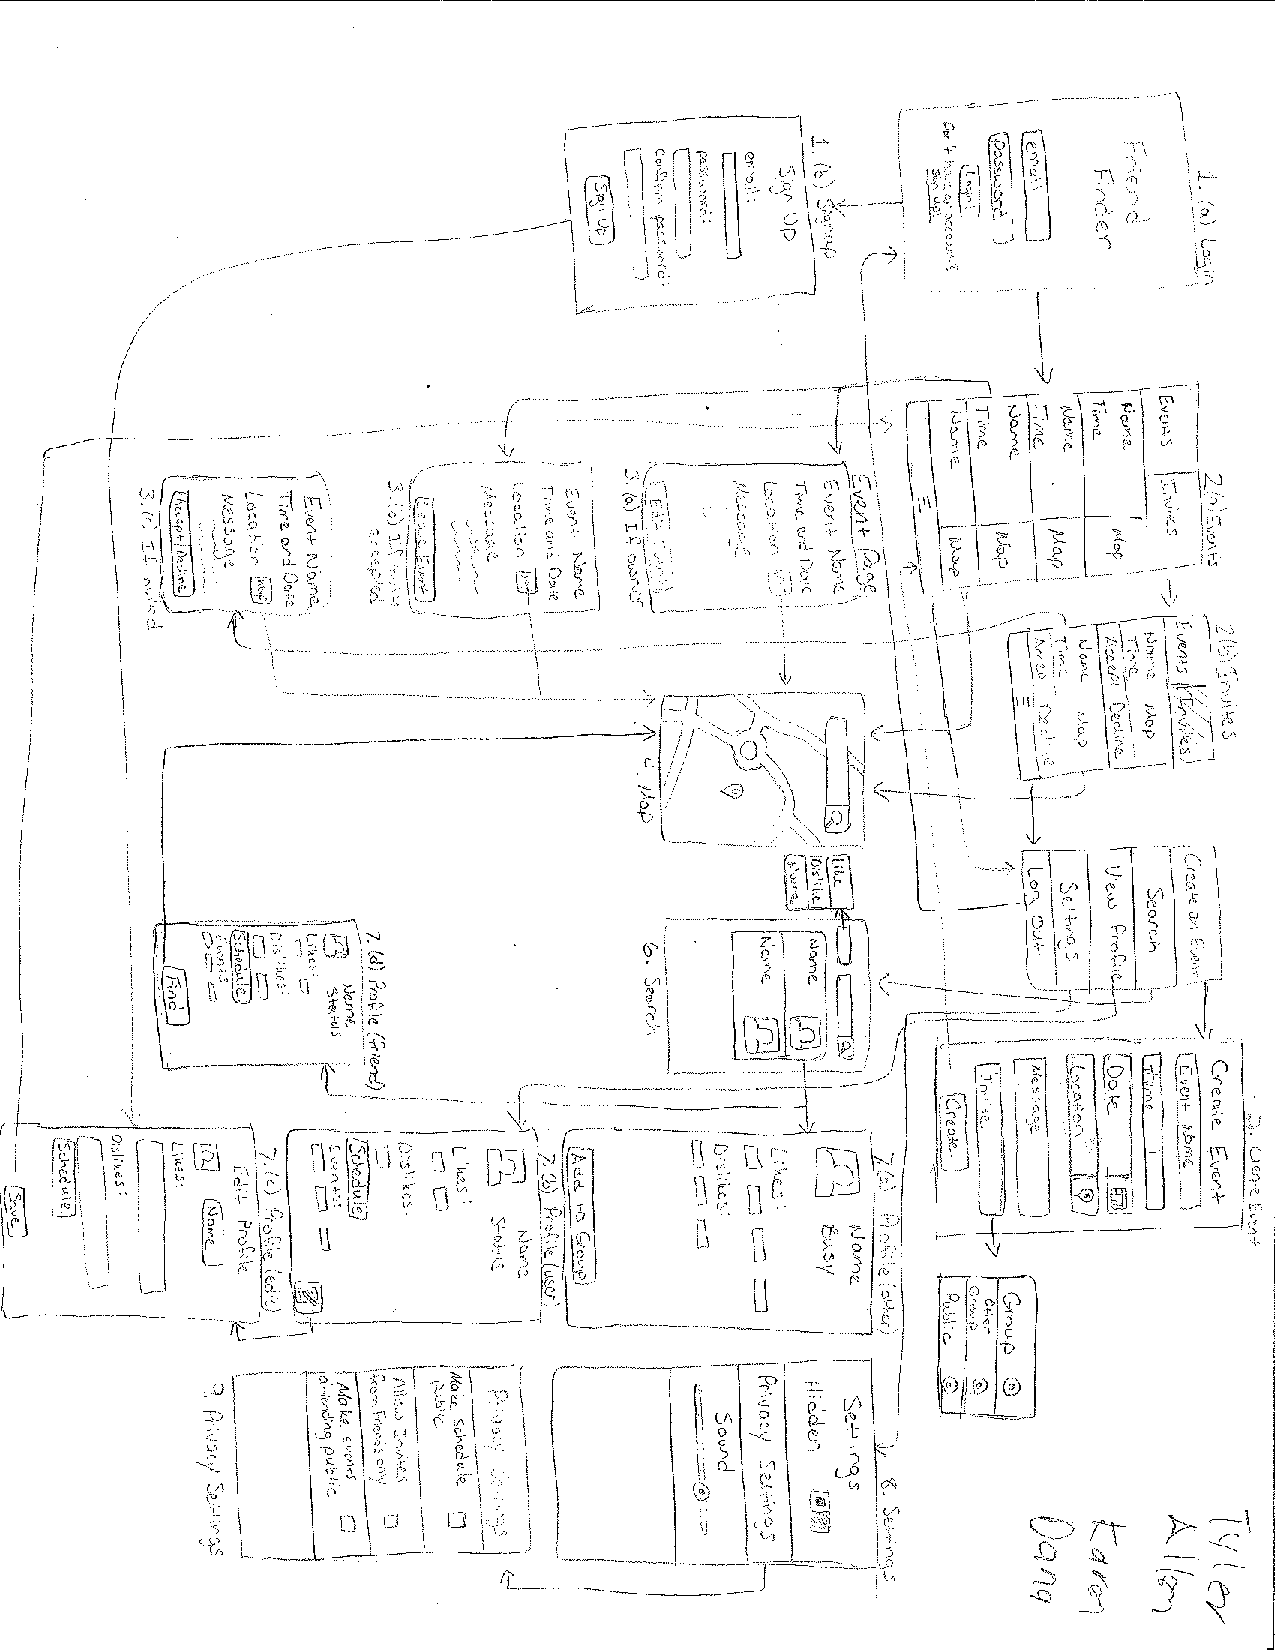
\includegraphics[scale=.2]{storyboard.pdf}
%\end{center}
%\end{frame}

\begin{frame}{Server UML Class Diagram}
\begin{center}
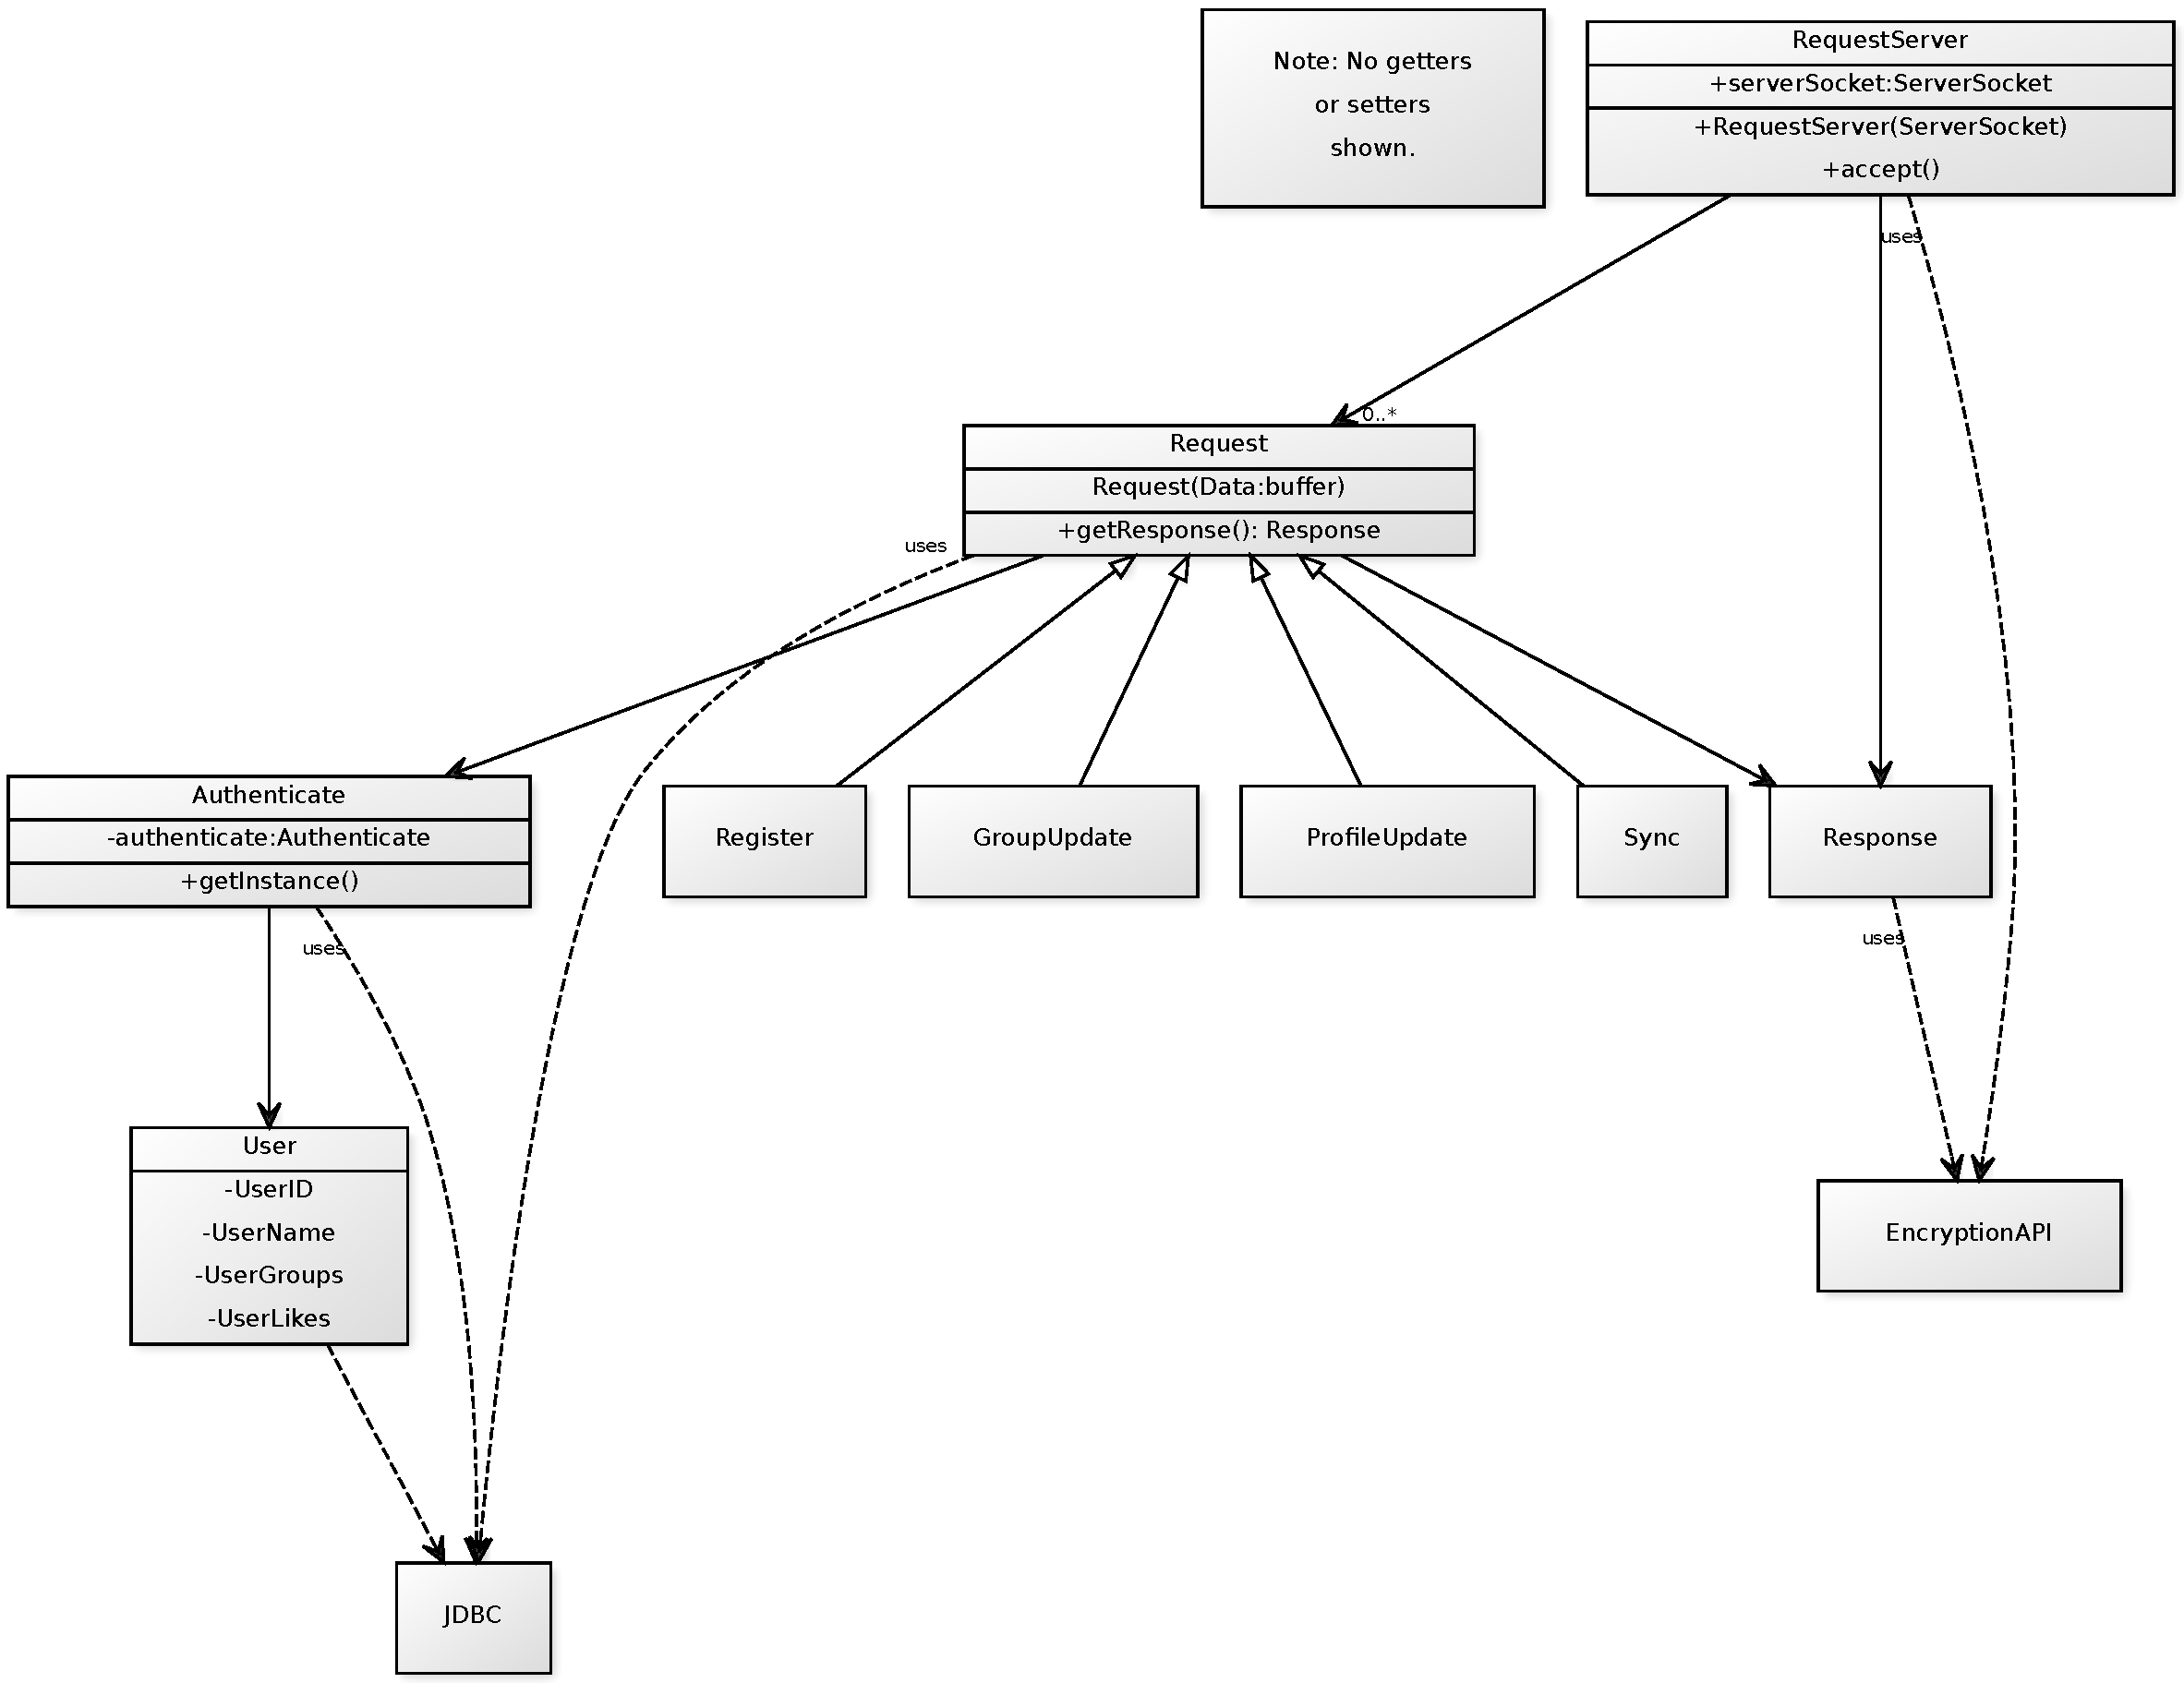
\includegraphics[scale=.2]{server.pdf}
\end{center}
\end{frame}

\begin{frame}{Application UML Class Diagram}
\begin{center}
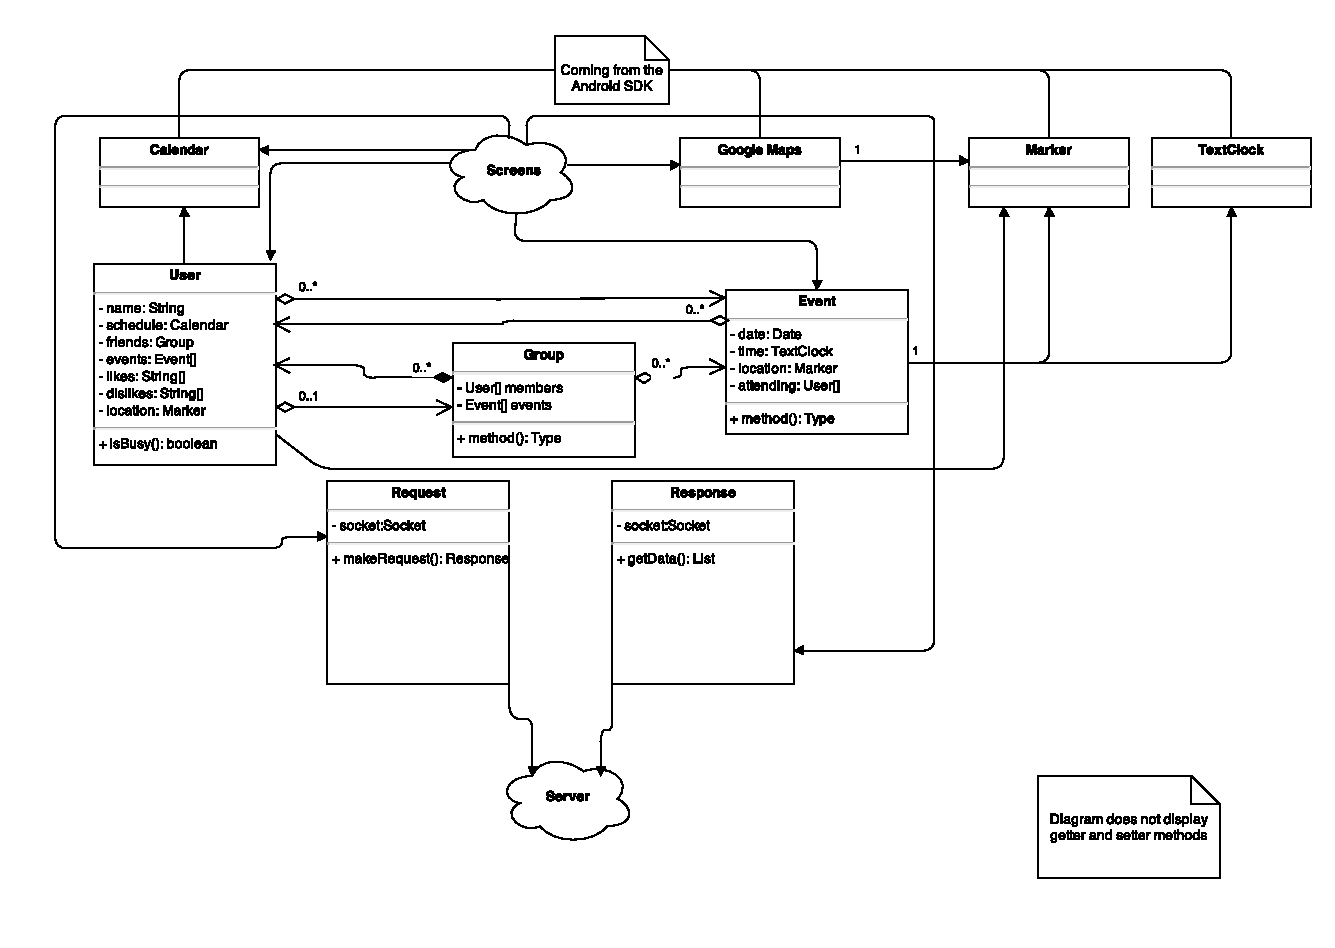
\includegraphics[scale=.4]{application.pdf}
\end{center}
\end{frame}

\begin{frame}{Current Implementation}
\begin{itemize}
\item Active development server with functioning test PostgresQL database.
\item Client-server communication via Transfer Control Protocol (TCP) and SSL is functioning.
\item Client has functioning \emph{ContentProvider} with SQLite Database containing the relevant
subset of daa received from the server.
\item Layout navigation primarily complete.
\item Viewing of events, groups, and users is complete.
\item Searching for users and groups are available. 
\item User login, authentication, and registration is complete.
\end{itemize}
\end{frame}

\begin{frame}{Demonstration}
\end{frame}

\section{Summary}
\begin{frame}{Summary}
\begin{itemize}
\item The communication and data storage backbone of the application has been completed.
\item A number of viewing, querying, and searching features have been implemented.
\item User authentication and registration has been completed.
\end{itemize}
\end{frame}

\begin{frame}{Future Work}
\begin{itemize}
\item Allow users to create their own groups, events, etc.
\item Add friends.
\item Allow users to set their schedule and make it viewable exclusively to friends.
\item Marking event locations on a Google Maps interface for other users to see. 
\item Allow syncing to be less redundant, more efficient.
\end{itemize}
\end{frame}

%\begin{frame}{References}
%\bibliography{friendfinder}
%\nocite{*}
%\end{frame}



\end{document}
